\documentclass[11pt]{article}
\usepackage[a4paper,margin=1in]{geometry}
\usepackage{amsmath,amssymb,amsthm,mathtools}
\usepackage{booktabs}
\usepackage{enumitem}
\usepackage{float}
\usepackage{graphicx}
\usepackage{hyperref}
\usepackage[nameinlink,capitalise]{cleveref}
\usepackage[numbers,sort&compress]{natbib}

\newtheorem{theorem}{Theorem}[section]
\newtheorem{proposition}[theorem]{Proposition}
\newtheorem{corollary}[theorem]{Corollary}
\newtheorem{remark}[theorem]{Remark}
\newcommand{\norm}[1]{\left\lVert#1\right\rVert}
\newcommand{\tr}{\operatorname{tr}}

\title{Physical-Covariance Block Residual Envelopes\\
\large Directional Sharpness versus Global Positive Size}
\author{Liang Wang}
\date{July 2026}

\begin{document}
\maketitle

\begin{abstract}
RH-66 repaired catastrophic packetwise scalarization by constructing a
block Krylov center and a positive-semidefinite residual Gram envelope.  Its
trace-global choice of scalar weights was still conservative in a specially
cancelling physical coefficient direction.  This paper optimizes those
weights for a prescribed positive coefficient covariance $W$.

If $P_1,\ldots,P_m\succeq0$ are the propagated block residual pieces and
\[
 \mathcal C(\theta)=\sum_i\frac{P_i}{\theta_i},
 \qquad \theta_i>0,\quad\sum_i\theta_i=1,
\]
then
\[
 \theta_i^*=
 \frac{\sqrt{\tr(WP_i)}}{\sum_j\sqrt{\tr(WP_j)}},
 \qquad
 \min_\theta\tr(W\mathcal C(\theta))
 =\left(\sum_i\sqrt{\tr(WP_i)}\right)^2.
\]
The Young parameter joining center and residual has an analogous exact
formula.  In the rank-one limit $W=uu^*$, the covariance objective is exactly
the RH-66 directional center-radius upper.  A strictly positive regularization
$W_\varepsilon=uu^*+\varepsilon(I-uu^*)$ keeps a globally valid PSD matrix.

We prove a sharpness--size duality.  If the physical ray annihilates every
residual piece, its excess is $O(\sqrt\varepsilon)$ while the off-ray global
envelope is $\Omega(\varepsilon^{-1/2})$.  On the exact cancellation witness,
the isotropic physical/global gains are $2.92454/1.16077$; at
$\varepsilon=10^{-24}$ they become $1.001027/489.96$.  Both rows are
certified with 256-bit Arb arithmetic.  On generic nonnormal and complex-phase
models, covariance focusing converges to the directional optima $3.89914$ and
$1.28847$ without a comparable global blow-up.

Factor-first evaluation in the physical coefficient frame removes a
binary64 cancellation artifact in RH-66: its archived gain $410.16$ is not
the mathematical isotropic gain of the exact witness.  The block theorem
remains valid; the stable factor-first evaluation gives $2.92454$.  The next
gate is uniform block depth and a production derivation of the physical
coefficient covariance.  No Stage A1 closure, arithmetic trace formula, or
Hilbert--Polya conclusion is claimed.
\end{abstract}

\noindent\textbf{Keywords:} coefficient covariance; positive-semidefinite
envelope; block Krylov method; phase cancellation; Gram factorization.

\medskip
\noindent\textbf{MSC 2020:} 47A10; 47B65; 65F35; 90C25; 93B07.

\section{Introduction}

RH-66 produced two block certificates: a sharp center-radius bound for one
physical coefficient vector and a PSD Gram bound valid for all packet
coefficients \citep{WangBlockGram2026}.  The latter is needed whenever a
downstream argument requires positivity before the physical coefficient has
been inserted.  Its scalar Cauchy and Young weights were chosen to minimize
ordinary trace, which treats every coefficient direction equally.

The physical packet fusion is not isotropic.  It comes with one selected
phase vector, or more generally a small ensemble of admissible phase vectors.
This suggests replacing trace by a positive covariance-weighted trace.  The
resulting problem is elementary convex optimization
\citep{BoydVandenberghe2004}, but it reveals a useful structural boundary:
directional sharpness is compatible with global PSD validity, yet exact
annihilation forces the globally valid matrix to become large away from the
physical ray.

\subsection*{Contributions and boundary}

\begin{enumerate}[leftmargin=2.2em]
 \item We solve exactly the covariance-weighted residual and Young parameter
       optimizations.
 \item We prove convergence to the rank-one directional certificate and a
       sharpness--global-size tradeoff for exact residual annihilation.
 \item We formulate a factor-first coefficient frame that avoids catastrophic
       cancellation when Grams contain large opposing entries.
 \item We audit one exact and two generic block models, including a 256-bit
       interval certificate for the exact tradeoff.
\end{enumerate}

The covariance is an input to this paper.  It has not yet been derived from
the production folded-Gaussian packet family.

\section{Covariance-optimal residual weights}
\label{sec:weights}

RH-66 writes the block remainder Gram as a positive upper built from finitely
many pieces $P_i\succeq0$.  The index $i$ includes the propagated Galerkin
residuals and the source reconstruction residual.  For
\begin{equation}
 \theta_i>0,qquad\sum_{i=1}^m\theta_i=1,
 \label{eq:simplex}
\end{equation}
put
\begin{equation}
 \mathcal C(\theta)=\sum_{i=1}^m\frac{P_i}{\theta_i}.
 \label{eq:residual-envelope}
\end{equation}
Every such choice is a valid PSD residual envelope.

\begin{theorem}[Covariance-optimal residual allocation]
\label{thm:residual-optimum}
Let $W\succ0$ and discard only identically zero $P_i$.  Define
$p_i=\tr(WP_i)>0$.  Then the unique minimizer of
$\tr(W\mathcal C(\theta))$ under \eqref{eq:simplex} is
\begin{equation}
 \theta_i^*=\frac{\sqrt{p_i}}{\sum_j\sqrt{p_j}},
 \label{eq:theta-optimum}
\end{equation}
and
\begin{equation}
 \min_\theta\tr(W\mathcal C(\theta))
 =\left(\sum_i\sqrt{p_i}\right)^2.
 \label{eq:residual-value}
\end{equation}
\end{theorem}

\begin{proof}
Weighted Cauchy gives
\[
 \left(\sum_i\sqrt{p_i}\right)^2
 =\left(\sum_i\sqrt{p_i/\theta_i}\sqrt{\theta_i}\right)^2
 \le\sum_i\frac{p_i}{\theta_i}.
\]
Equality holds exactly when $\theta_i\propto\sqrt{p_i}$.
\end{proof}

Let $Y\succeq0$ be the center Gram.  RH-66 then uses
\begin{equation}
 \mathcal G(\eta,\theta)
 =(1+\eta)Y+(1+\eta^{-1})\mathcal C(\theta),
 \qquad \eta>0.
 \label{eq:full-envelope}
\end{equation}

\begin{proposition}[Covariance-optimal Young parameter]
\label{prop:young}
For fixed $\theta$, put
$y=\tr(WY)$ and $c=\tr(W\mathcal C(\theta))$.  If $y,c>0$, then
\begin{equation}
 \eta^*=\sqrt{c/y},
 \qquad
 \min_\eta\tr(W\mathcal G(\eta,\theta))
 =(\sqrt y+\sqrt c)^2.
 \label{eq:eta-optimum}
\end{equation}
The zero cases are obtained as one-sided limits.
\end{proposition}

\begin{proof}
The variable part is $\eta y+c/\eta$, whose arithmetic--geometric mean
minimum is $2\sqrt{yc}$.
\end{proof}

These optimizations do not weaken global validity.  They select scalar
weights inside the same Loewner upper proved by RH-66.

\section{Rank-one limit and the global-size price}
\label{sec:tradeoff}

Let $u$ be a unit physical coefficient vector and
$P_\perp=I-uu^*$.  Consider
\begin{equation}
 W_\varepsilon=uu^*+\varepsilon P_\perp,
 \qquad 0<\varepsilon\le1.
 \label{eq:regularized-covariance}
\end{equation}

\begin{proposition}[Directional rank-one limit]
\label{prop:rank-one}
If every nonzero residual piece has $u^*P_iu>0$, then as
$\varepsilon\downarrow0$, the weights in \eqref{eq:theta-optimum}, the Young
parameter, and the physical value $u^*\mathcal G u$ converge to the RH-66
directional center-radius optimum.  The envelope remains bounded.
\end{proposition}

\begin{proof}
All scores
$\tr(W_\varepsilon P_i)=u^*P_iu+\varepsilon\tr(P_\perp P_i)$ converge to
strictly positive limits.  Hence the formulas in
\cref{thm:residual-optimum,prop:young} are continuous.  At
$W_0=uu^*$, \eqref{eq:residual-value} is precisely the square of the sum of
the directional residual radii.
\end{proof}

Exact cancellation is a boundary case, not covered by strict positivity.

\begin{theorem}[Sharpness--global-size duality]
\label{thm:duality}
Assume
\begin{equation}
 P_iu=0\quad(1\le i\le m),
 \qquad Yu=Gu,
 \qquad y_0=u^*Yu>0,
 \label{eq:exact-annihilation}
\end{equation}
where $G$ is the exact Gram.  Suppose the complement residual envelope is
nonzero.  Then the covariance-optimal residual weights are independent of
$\varepsilon$, and
\begin{equation}
 \eta_\varepsilon=\Theta(\sqrt\varepsilon),
 \qquad
 \frac{u^*\mathcal G_\varepsilon u}{u^*Gu}
 =1+\Theta(\sqrt\varepsilon),
 \qquad
 \norm{\mathcal G_\varepsilon}
 =\Omega(\varepsilon^{-1/2}).
 \label{eq:duality-rates}
\end{equation}
\end{theorem}

\begin{proof}
Positivity and $u^*P_iu=0$ imply $P_iu=0$.  Every covariance score is
$\varepsilon\tr(P_\perp P_i)$, so the common factor cancels from
\eqref{eq:theta-optimum}; call the resulting nonzero envelope
$\mathcal C_\perp$.  Therefore
\[
 \eta_\varepsilon=
 \sqrt{\frac{\varepsilon\tr(P_\perp\mathcal C_\perp)}
 {y_0+\varepsilon\tr(P_\perp Y)}}.
\]
Since $\mathcal C_\perp u=0$, the physical value is
$(1+\eta_\varepsilon)y_0$.  On the complement, the term
$(1+\eta_\varepsilon^{-1})\mathcal C_\perp$ has norm of order
$\eta_\varepsilon^{-1}$.
\end{proof}

Thus no contradiction exists between a sharp physical ray and a large
global PSD matrix.  The large off-ray value is the price of requiring one
matrix to remain valid for coefficient directions the physical covariance
assigns almost zero weight.

\section{Factor-first coefficient frames}
\label{sec:frame}

Let $U=[u,U_\perp]$ be unitary.  Mathematically one may transform a Gram by
$U^*GU$.  Numerically, this can subtract large nearly equal entries after
they have already been squared.  The implementation instead transforms each
factor first:
\begin{equation}
 (XU)^*M(XU),
 \label{eq:factor-first}
\end{equation}
for the exact response, center, and every residual factor.  This preserves
structural zeros before Gram formation and is substantially more stable in
the cancellation witness.

This point corrects a finite-precision diagnostic in RH-66.  The archived
$410.16$ uniform-Gram gain was a valid but severely rounded binary64 upper
formed in the original packet coordinates.  The exact scalar reduction and
256-bit audit below give the mathematical isotropic gain $2.92454$.  No
analytic RH-66 statement changes.

\section{Model audit}
\label{sec:audit}

The exact witness uses the RH-66 diagonal model.  In the physical frame, its
target and complement decouple.  If $y$ is the exact target energy,
$Y_\perp$ the complement center, and $C_\perp$ the optimized residual upper,
then
\begin{equation}
 \eta_\varepsilon=
 \sqrt{\frac{\varepsilon C_\perp}{y+\varepsilon Y_\perp}},
 \qquad
 \text{physical gain}=1+\eta_\varepsilon.
 \label{eq:exact-ledger}
\end{equation}
Here
\[
 y=6.92944\times10^{-17},\quad
 Y_\perp=19.7435,\quad C_\perp=73.1273,
\]
so the asymptotic regime begins only below approximately $10^{-18}$.

\begin{table}[H]
\centering
\caption{Covariance sharpness and global positive size.}
\label{tab:tradeoff}
\begin{tabular}{lrrr}
\toprule
model / $\varepsilon$ & physical gain & weighted gain & global gain\\
\midrule
exact cancellation / $1$       & 2.924544 & 1.160769 & 1.160769\\
exact cancellation / $10^{-24}$& 1.001027 & 1.002054 & 489.960\\
exact cancellation / $10^{-28}$& 1.000010 & 1.000021 & $4.8933\times10^4$\\
nonnormal chain / $1$           & 3.950049 & 4.004647 & 3.851919\\
nonnormal chain / $10^{-10}$    & 3.899145 & 3.899145 & 3.934330\\
complex phase / $1$             & 1.295052 & 1.343557 & 1.169230\\
complex phase / $10^{-10}$      & 1.288471 & 1.288471 & 1.154899\\
\bottomrule
\end{tabular}
\end{table}

The generic models satisfy the strict case of \cref{prop:rank-one}.  Their
physical values converge rapidly to the directional optima $3.8991448$ and
$1.2884708$, while the global spectral gains remain bounded.  The computed
PSD slack is positive on all rows.

\begin{figure}[H]
\centering
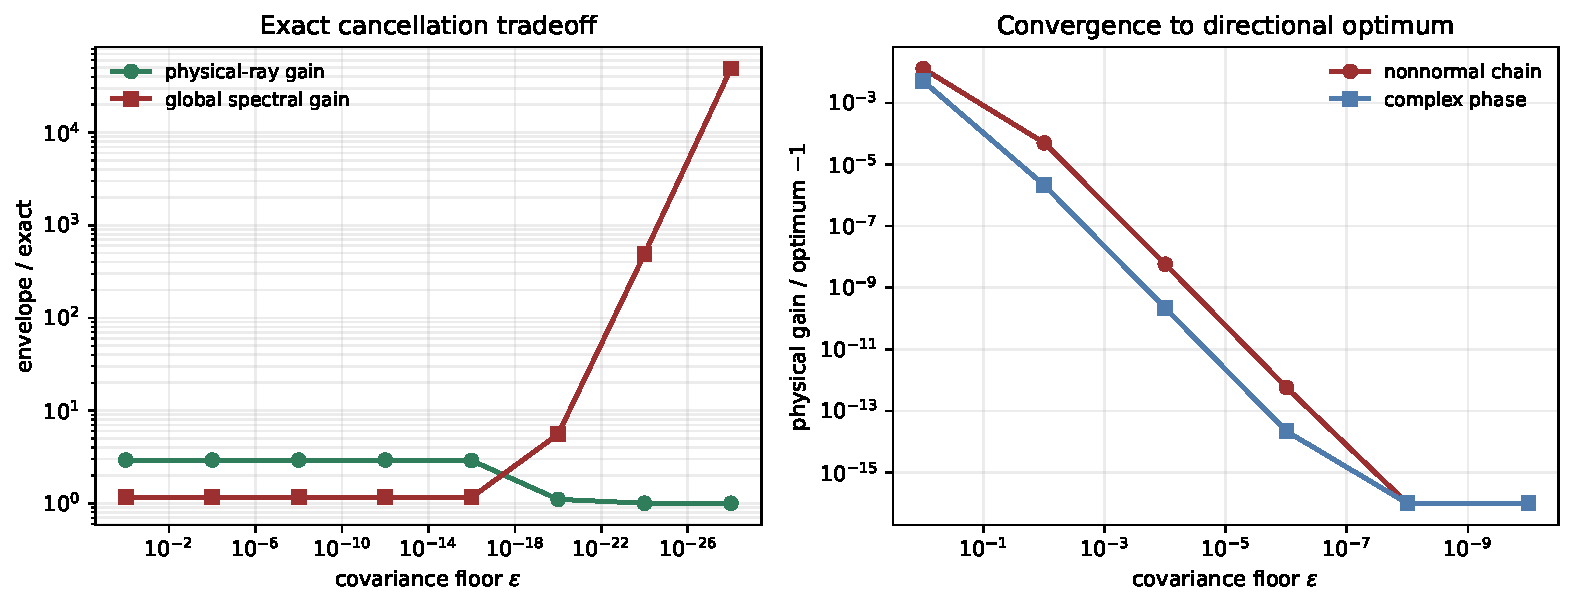
\includegraphics[width=0.98\textwidth]{figures/physical_covariance_block_envelopes.pdf}
\caption{Left: the exact cancellation ray becomes sharp only by enlarging the
off-ray global envelope.  Right: generic models converge rapidly to their
directional optima without that singular tradeoff.}
\label{fig:tradeoff}
\end{figure}

A 256-bit Arb audit certifies the exact scalar ledger.  At
$\varepsilon=1$, the physical gain lies in $(2,3)$ and the global gain is
below $1.2$.  At $\varepsilon=10^{-24}$, the physical gain lies in
$(1.001,1.002)$ while the global gain exceeds $400$.

\section{Route consequence}
\label{sec:route}

The PSD-envelope wall is now classified rather than merely observed:

\begin{enumerate}[leftmargin=2.2em]
 \item for generic physical directions, covariance focusing recovers the
       directional block certificate with bounded global cost;
 \item exact annihilation directions force a tradeoff between physical
       sharpness and global PSD size;
 \item stable factor-first coordinates are mandatory before deciding which
       regime is present.
\end{enumerate}

This leaves two analytic inputs.  First, the physical packet construction
must supply an admissible covariance $W_\sigma$ or prove that one selected ray
is sufficient downstream.  Second, the required block Krylov depth must be
controlled uniformly.  RH-68 should therefore audit uniform depth and prove
a no-go theorem if a growing family of separately visible modes forces the
rank to grow.

\section{No arithmetic or Hilbert--Polya conclusion}

This paper constructs no self-adjoint operator, no $T\log T$ counting law,
no prime-power trace formula, and no completed-zeta identity.  It makes no
Hilbert--Polya or Riemann-hypothesis claim.  Stage A1 and unconditional Stage
A4 remain open.

\section{Reproducibility}

The directory contains covariance optimization code, tests, exact and
generic pilots, the Arb audit, figures, hashes, and publication artifacts.
The main commands are:
\begin{verbatim}
pytest -q -p no:cacheprovider
python experiments/run_covariance_envelope_pilot.py
python experiments/run_arb_covariance_tradeoff.py
MPLBACKEND=Agg python experiments/make_figures.py
latexmk -pdf -interaction=nonstopmode -halt-on-error main.tex
\end{verbatim}

The optimization identities and tradeoff theorem are analytic.  The generic
model rows are binary64 evidence; the exact cancellation rows have a 256-bit
audit.  Production covariance derivation, uniform block depth, Stage A1,
unconditional Stage A4, a self-adjoint Hilbert--Polya operator, an arithmetic
trace formula, and a zeta-zero identity remain open.

\bibliographystyle{plainnat}
\bibliography{references}
\end{document}
